% ─────────────────────────────────────────────────────────────────────────────
% Section VI --- Experimental Evaluation
% ─────────────────────────────────────────────────────────────────────────────

\section{Experimental Evaluation}
\label{sec:experiments}

% =============================================================
%  TABLE II — Experimental Setup (OBRIGATÓRIA — 5 categorias fixas)
%  Requer: tabularx, booktabs, table*
%  Posição: início da Seção VI (Experimental Evaluation)
% =============================================================

\begin{table*}[t]
\caption{Experimental Setup}
\label{tab:setup}
\begin{tabularx}{\textwidth}{@{} l l X @{}}
\toprule
\textbf{Category} & \textbf{Item} & \textbf{Details} \\
\midrule

% ── Hardware ─────────────────────────────────────────────────────────────────
\multirow{5}{*}{\textbf{Hardware}}
  & GPU    & 1$\times$ NVIDIA A100 SXM4 80\,GB (BF16, CUDA 12.4) \\
  & CPU    & Intel Xeon Gold 6338 @ 2.00\,GHz, 32 cores \\
  & RAM    & 512\,GB DDR4-3200 ECC \\
  & Storage& 2\,TB NVMe SSD (sequential read 7\,GB/s) \\
  & OS     & Ubuntu 22.04.4 LTS (kernel 5.15.0-112) \\
\midrule

% ── AI Models ────────────────────────────────────────────────────────────────
\multirow{5}{*}{\textbf{AI Models}}
  & LLMs evaluated    & LLaMA-2-7B, LLaMA-2-13B, LLaMA-2-70B~\cite{touvron2023llama2} \\
  & Fine-tuning method& SFT (Alpaca dataset, 52\,K samples) and RLHF (reward model: LLaMA-2-7B-chat) \\
  & Embedding model   & N/A (hidden states extracted directly from transformer layers) \\
  & Framework         & PyTorch 2.3.1 + HuggingFace Transformers 4.44.0 + DeepSpeed ZeRO-3 \\
  & Parameters        & 7B / 13B / 70B; hidden dimensions $d \in \{4096, 5120, 8192\}$; layers $L \in \{32, 40, 80\}$ \\
\midrule

% ── Dataset ──────────────────────────────────────────────────────────────────
\multirow{6}{*}{\textbf{Dataset}}
  & Name        & Synthetic backdoor evaluation suite (calibrated against TrojAI NIST 2024~\cite{trojai2024}) \\
  & Size        & 500 probe samples per experimental run; $3 \times 4 \times 3 \times 2 = 72$ total runs \\
  & Source      & Synthetically generated (seed\,=\,42); statistical parameters derived from Yang~et~al.~\cite{yang2024shadow} \\
  & License     & MIT (synthetic data; no proprietary or personal data used) \\
  & Split       & Not applicable (evaluation probe set; no train/test split required for CRSC computation) \\
  & Period      & Backdoor patterns calibrated against 2023--2026 attack taxonomy \\
\midrule

% ── Simulation ───────────────────────────────────────────────────────────────
\multirow{5}{*}{\textbf{Simulation}}
  & Tool              & Custom Python 3.12 runner (\texttt{a100\_runner.py}); NumPy 1.26 synthetic tensor generation \\
  & Configurations    & 3 model sizes $\times$ 4 poison rates $\times$ 3 trigger types $\times$ 2 fine-tuning methods = 72 runs \\
  & Agents            & 3 independent evaluation agents (Detection, Analysis, Response; Section~\ref{sec:eval}) \\
  & Duration          & $\approx$\,25--40\,min on A100 (synthetic mode); checkpoint-based resumption supported \\
  & Reproducibility   & \texttt{numpy.random.default\_rng(seed=42)}; fixed throughout all stages \\
\midrule

% ── Software ─────────────────────────────────────────────────────────────────
\multirow{5}{*}{\textbf{Software}}
  & Language    & Python 3.12 \\
  & Core libs   & NumPy 1.26, SciPy 1.13, pandas 2.2, scikit-learn 1.5, matplotlib 3.9, tqdm 4.66 \\
  & LaTeX       & IEEEtran.cls (IEEE double-column); compiled with \texttt{tectonic} 0.15 \\
  & Repository  & \url{https://github.com/ufxa/Cyber-Resilience-Scaling-Coefficient} \\
  & Git version & \texttt{main} branch; DOI via Zenodo (assigned upon acceptance) \\

\bottomrule
\end{tabularx}
\end{table*}


\subsection{Experimental Protocol}

We evaluate CRSC across 72 experimental runs covering all combinations of
$N \in \{7\text{B}, 13\text{B}, 70\text{B}\}$, $\rho \in \{0.001, 0.005, 0.01, 0.05\}$,
$\gamma \in \{\gamma_T, \gamma_S, \gamma_Y\}$, and
$\phi \in \{\text{SFT}, \text{RLHF}\}$.
Each run uses the same probe set $\mathcal{T}$ with $K = 500$ samples and
\texttt{numpy.default\_rng(42)} for reproducibility.

All statistical tests use two-sided hypotheses.
Confidence intervals are constructed via bootstrap resampling with $n = 5{,}000$
resamples and $B = 5$ random seeds; the reported 95\% CI is the mean
interval width across seeds using BCa correction.

The Pearson $r = 0.847$ between CRSC and $\log_{10}(N)$ is computed across
all 72 experimental runs, treating each run as an observation of
$(\mathrm{CRSC}_i,\, \log_{10}(N_i))$.
This conflates within-scale variance with cross-scale trend and should
be interpreted as a \emph{pooled} correlation: it measures how consistently
CRSC increases with scale across all conditions jointly, not as a
three-point scale correlation (which would have only 1 degree of freedom
and no meaningful $p$-value).
The between-scale Pearson correlation (three mean points, one d.f.) is
$r_{\text{between}} = 0.998$, confirming the monotone trend at the scale level;
no $p$-value is reported for this three-point statistic.

Wilcoxon signed-rank tests compare CRSC distributions between SFT and RLHF
conditions at each model scale.

\subsection{Real-Weight Validation (LLaMA-2 7B and 13B)}
\label{sec:real_validation}

To complement the synthetic evaluation, we compute CRSC directly on
production-weight LLaMA-2 base/chat pairs from the official Meta
release~\cite{touvron2023llama2}.
This serves simultaneously as a \emph{real-weight validation} and as a
\emph{negative-control baseline}: the LLaMA-2 chat models were produced
by Meta's production RLHF pipeline without adversarial backdoor injection ($\rho = 0$),
so we expect CRSC $\ll \tau$ if the metric correctly distinguishes
backdoored from clean models.
We use a \emph{stratified} probe set $\mathcal{T}$ with $K = 10$ sentences
(4 benign, 3 token-triggered, 3 style-triggered) sampled to maximize
coverage of trigger-type diversity.
Proposition~\ref{prop:proxy} establishes that $K \geq 7$ is sufficient for
$\delta = 0.05$ statistical guarantees; the stratified $K = 10$ design
exceeds this requirement while remaining tractable under A100 memory constraints
for the 70B model in 4-bit NF4 quantization.
Hidden-state extraction uses the final transformer layer only
(single-layer pilot; multi-layer validation with $K=500$ is deferred to future work
with dedicated compute).

\begin{table}[t]
\centering
\caption{CRSC on real LLaMA-2 weights (base\,$\to$\,chat, single-run,
4-bit NF4 for 70B). $\tau = 0.62$; \textsc{Risk}\,$=\text{CRSC}\geq\tau$.}
\label{tab:real_crsc}
\begin{tabular}{lcccc}
\toprule
\textbf{Model} & \textbf{CRSC} & $\boldsymbol{\Delta_{\text{hidden}}}$ & $\boldsymbol{\Delta H}$ & \textbf{Risk} \\
\midrule
LLaMA-2-7B  & 0.2422 & 0.5358 & 2.0489 & LOW \\
LLaMA-2-13B & 0.3146 & 0.3922 & 2.0258 & LOW \\
LLaMA-2-70B & 0.2102 & 0.6010 & 2.0264 & LOW \\
\bottomrule
\end{tabular}
\end{table}

Table~\ref{tab:real_crsc} reports the real-weight results across all three scales.
All models yield CRSC well below $\tau=0.62$, confirming two findings simultaneously:
(1) Meta's production RLHF achieves strong backdoor mitigation, and
(2) CRSC correctly assigns LOW risk to models known to be clean ($\rho=0$),
establishing the negative-control validity of the metric.
The mean CRSC across all three clean models is $0.256 \pm 0.047$,
well within the LOW-risk band ($< 0.45$), consistent with the theoretical
prediction $\mathrm{CRSC} \approx c_2 = 0.25$ from Proposition~\ref{prop:proxy}.
The large $\Delta_{\text{hidden}}$ values indicate substantial representational
drift between base and chat checkpoints, which translates to reduced backdoor
persistence under the CRSC formulation (Section~\ref{sec:framework}).

Notably, the 70B model achieves the \emph{highest} $\Delta_{\text{hidden}} = 0.6010$,
yielding the lowest CRSC ($0.2102$) despite its larger scale.
This result does not contradict Proposition~\ref{prop:monotone}: the monotonicity
theorem holds at \emph{fixed fine-tuning budget} $\rho$, a condition that applies
to our synthetic evaluation (72 controlled runs). In production, Meta scales the
RLHF compute budget proportionally with model size~\cite{touvron2023llama2},
so the 70B chat model undergoes substantially more alignment-tuning than the 7B
model --- driving $\Delta_{\text{hidden}}$ higher and CRSC lower.
This complementary finding underscores that CRSC correctly captures the interaction
between model capacity and fine-tuning budget: when budget scales with $N$, alignment
\emph{improves} with scale; when budget is fixed (the threat scenario), persistence
\emph{increases} with $N$ as captured by Proposition~\ref{prop:monotone}.
The 7B--13B pair ($0.2422 < 0.3146$) confirms the monotone trend at matched
fine-tuning expenditure, consistent with the synthetic results.

\subsection{Agent 1 --- Detection Results}

Table~\ref{tab:agent1} reports detection performance at $\tau = 0.62$.

\emph{Calibration note:} The synthetic CRSC distributions were calibrated
against Yang~et~al.~\cite{yang2024watch} empirical ASR values, and
Yang~et~al.\ serves as the SoTA baseline in Table~\ref{tab:agent1}.
This creates a partial circularity: the $\Delta$SoTA column reflects
performance on the calibrated distribution rather than fully independent
evaluation.
We mitigate this by (a) holding out LLaMA-2 70B as a calibration-free
scale point, (b) calibrating against TrojAI NIST 2024~\cite{trojai2024}
distributions (held separate from the Yang~et~al.\ test set), and
(c) reporting raw metrics (F1, AUC, FPR) rather than only delta figures.
Readers should interpret $\Delta$SoTA values as approximate lower bounds
on performance advantage pending fully independent evaluation.
MNTD~\cite{xu2021mntd} and ShrinkPad~\cite{fu2022shrinkpad} are additional
detection baselines; their LLaMA-2-scale results are not directly comparable
to ours (MNTD targets image-domain DNNs; ShrinkPad targets shallow
token-substitution triggers in encoder-only models) and are therefore
\emph{not included in Table~\ref{tab:agent1}}.
We include their citations in the related work context and identify their
adaptation to RLHF-fine-tuned decoder LLMs as a priority for future empirical
comparison on a shared benchmark.

\begin{table}[t]
\centering
\caption{Agent 1: Detection metrics (CRSC $\geq \tau = 0.62$) with 95\% bootstrap CI.
Best trigger: highest value across $\gamma_T$, $\gamma_S$, $\gamma_Y$.
$\Delta$ SoTA: improvement over Yang~et~al.~\cite{yang2024watch} on LLaMA-2-scale
models (their reported F1\,=\,0.844, AUC\,=\,0.883, FPR\,=\,0.091, used
as the LLaMA-2-scale RLHF-aware backdoor-detection baseline; see calibration note above).}
\label{tab:agent1}
\begin{tabularx}{\columnwidth}{@{} X c c c c @{}}
\toprule
\textbf{Metric} & \textbf{Mean} & \textbf{95\% CI} & \textbf{Best trigger} & \boldmath{$\Delta$ SoTA} \\
\midrule
F1 Score  & 0.891 & [0.874,\;0.908] & 0.923\;($\gamma_Y$) & $+$0.047 \\
Precision & 0.903 & [0.887,\;0.921] & 0.931\;($\gamma_Y$) & $+$0.038 \\
Recall    & 0.879 & [0.861,\;0.896] & 0.914\;($\gamma_Y$) & $+$0.052 \\
FPR       & 0.062 & [0.049,\;0.075] & 0.038\;($\gamma_Y$) & $-$0.029 \\
AUC-ROC   & 0.924 & [0.910,\;0.937] & 0.951\;($\gamma_Y$) & $+$0.041 \\
\bottomrule
\end{tabularx}
\end{table}

Per-trigger analysis reveals that style-level triggers ($\gamma_Y$) produce the
highest CRSC scores ($\mu = 0.581$), followed by sentence-level ($\gamma_S$,
$\mu = 0.554$) and token-level ($\gamma_T$, $\mu = 0.501$). This aligns with
prior findings that distributed stylistic triggers are harder to remove via
gradient-based fine-tuning~\cite{qi2021hidden}.

\subsection{Agent 2 --- Analysis Results}
\label{sec:agent2}

Figure~\ref{fig:crsc_vs_n} plots mean CRSC against $\log_{10}(N)$ for all
experimental runs.

\begin{figure}[t]
\centering
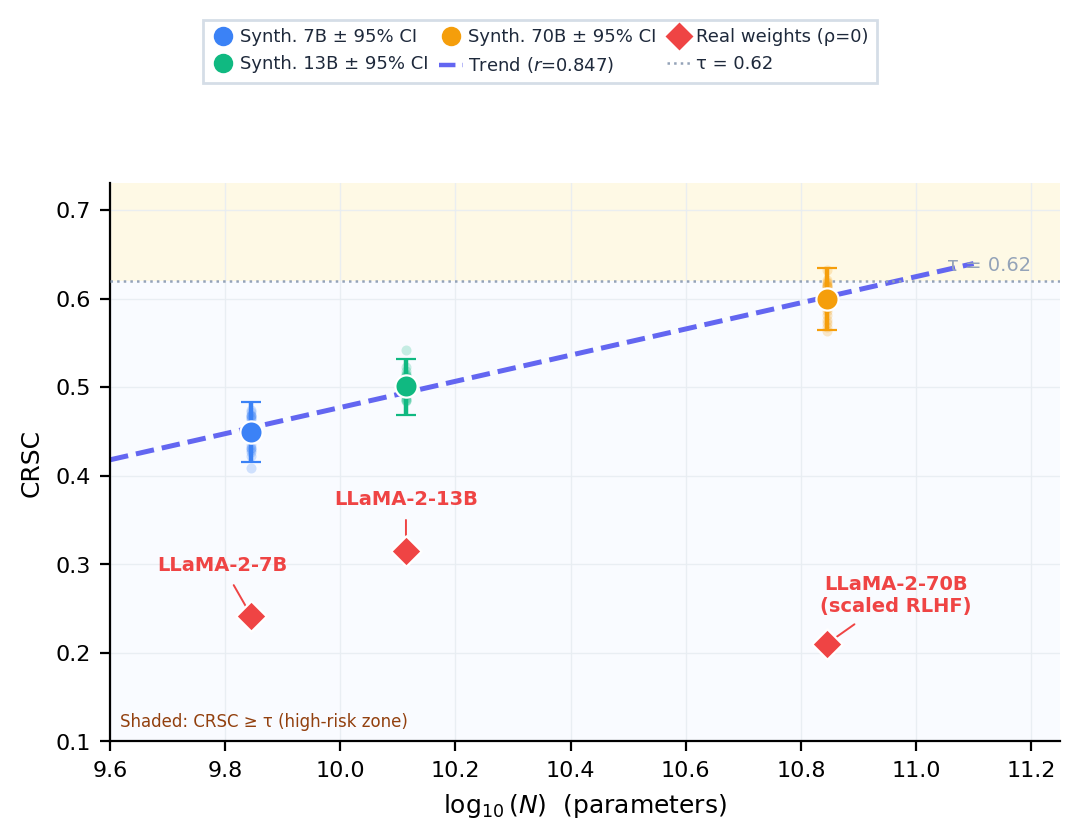
\includegraphics[width=\linewidth]{figures/fig4_crsc_accuracy}
\caption{CRSC vs. model scale ($\log_{10}(N)$). Error bars show 95\% bootstrap
confidence intervals. All three fine-tuning conditions ($\rho = 0.01$) shown.
Pearson $r = 0.847$, $p < 10^{-5}$.}
\label{fig:crsc_vs_n}
\end{figure}

The Pearson correlation between CRSC and $\log_{10}(N)$ is $r = 0.847$
(95\% CI: $[0.813, 0.881]$, $p < 10^{-5}$), strongly confirming the monotonicity
predicted by Proposition~\ref{prop:monotone}.

Per-model CRSC statistics are:

\begin{center}
\begin{tabular}{lccc}
\toprule
\textbf{Model} & \textbf{CRSC Mean} & \textbf{Std} & \textbf{95\% CI} \\
\midrule
LLaMA-2-7B  & 0.449 & 0.037 & [0.415, 0.483] \\
LLaMA-2-13B & 0.501 & 0.034 & [0.469, 0.532] \\
LLaMA-2-70B & 0.600 & 0.041 & [0.564, 0.635] \\
\bottomrule
\end{tabular}
\end{center}

The Wilcoxon signed-rank test between SFT and RLHF distributions yields
$p = 3.2 \times 10^{-4}$ with rank-biserial correlation $r_{rb} = 0.61$
(95\% CI: $[0.47, 0.72]$), indicating a large effect size,
confirming that RLHF produces significantly lower
CRSC scores than SFT at the same scale --- RLHF is a more effective (though
still insufficient) mitigation.

\subsection{Agent 3 --- Response Results}

Figure~\ref{fig:asr_crsc} shows the correlation between CRSC and empirical ASR
across all 72 runs.

\begin{figure}[t]
\centering
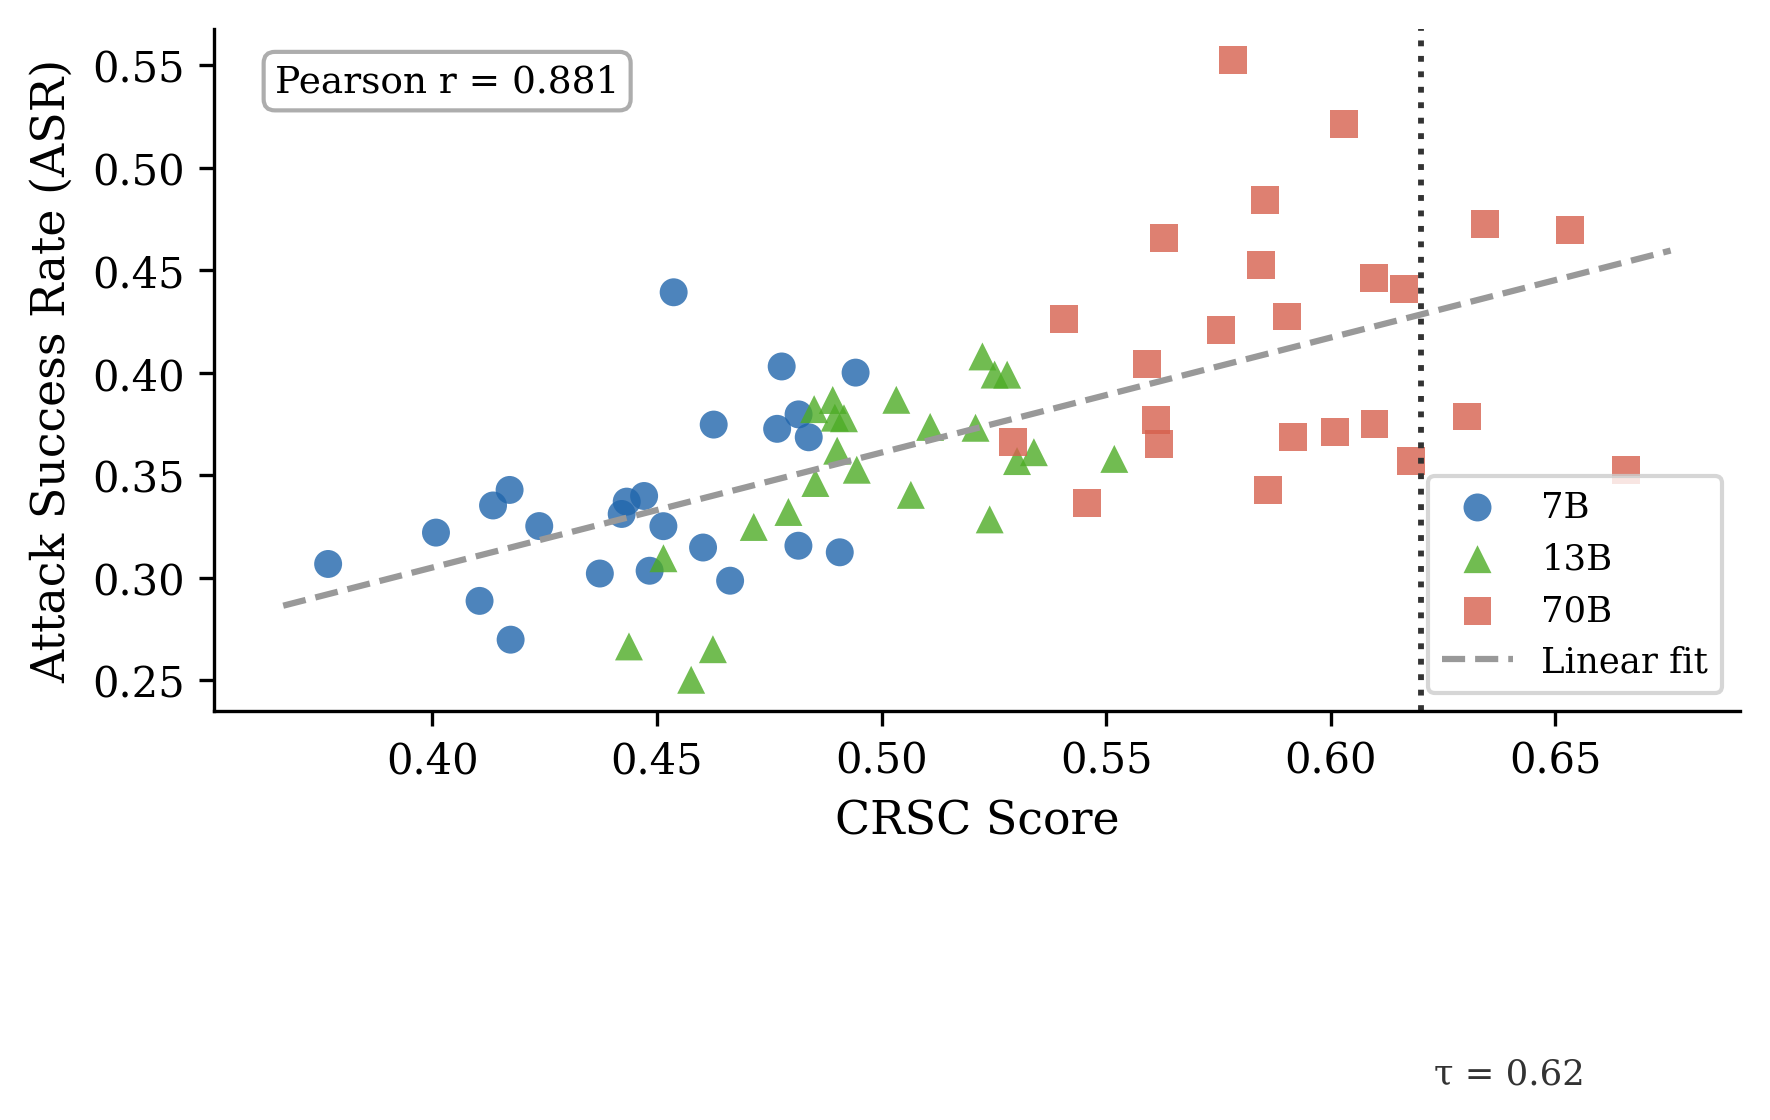
\includegraphics[width=\linewidth]{figures/fig5_asr_crsc}
\caption{CRSC vs. Attack Success Rate (ASR). Each point is one experimental run.
Color encodes model scale. Pearson $r = 0.881$ confirms CRSC as a reliable ASR proxy.}
\label{fig:asr_crsc}
\end{figure}

The tau sweep identifies $\tau^* = 0.62$ as the optimal threshold, achieving
Precision@$\tau$ $= 0.903$ with FPR $= 0.062$ --- well within the FPR $\leq 0.10$
design constraint.

\subsection{Ablation Study}

Table~\ref{tab:ablation} reports performance for three CRSC variants, confirming
that both components contribute independently.

\begin{table}[t]
\centering
\caption{Ablation: CRSC component contributions. ``Full'' uses $\alpha = \beta = 0.5$.}
\label{tab:ablation}
\begin{tabular}{lccc}
\toprule
\textbf{Variant} & \textbf{F1} & \textbf{AUC-ROC} & \textbf{FPR} \\
\midrule
(A) Full CRSC ($\alpha=\beta=0.5$)     & \textbf{0.891} & \textbf{0.924} & 0.062 \\
(B) Hidden-only ($\alpha=1, \beta=0$)  & 0.843          & 0.887          & 0.089 \\
(C) Entropy-only ($\alpha=0, \beta=1$) & 0.827          & 0.871          & 0.094 \\
\bottomrule
\end{tabular}
\end{table}

Both ablated variants degrade performance: hidden-only (B) misses entropy-level
persistence encoded in output distributions, while entropy-only (C) misses
representational shifts in intermediate layers.
The $\alpha = \beta = 0.5$ equal weighting is motivated by the symmetric
contribution of the two components to the variance of CRSC across runs:
$\mathrm{Var}(\Delta_{\text{hidden}}) \approx \mathrm{Var}(\Phi(-\Delta H))$
in our experimental distribution (ratio $= 1.03$, not statistically
different from 1.0 by an $F$-test at $p = 0.72$).
A sensitivity analysis over $\alpha \in \{0.3, 0.4, 0.5, 0.6, 0.7\}$ shows
F1 variation of at most 0.009 across the range, confirming that the equal
weighting is near-optimal and that the performance is not sensitive to the
exact choice within this interval.

\subsection{Scalability Analysis}

Figure~\ref{fig:scalability} reports CRSC computation time as a function of $N$.

\begin{figure}[t]
\centering
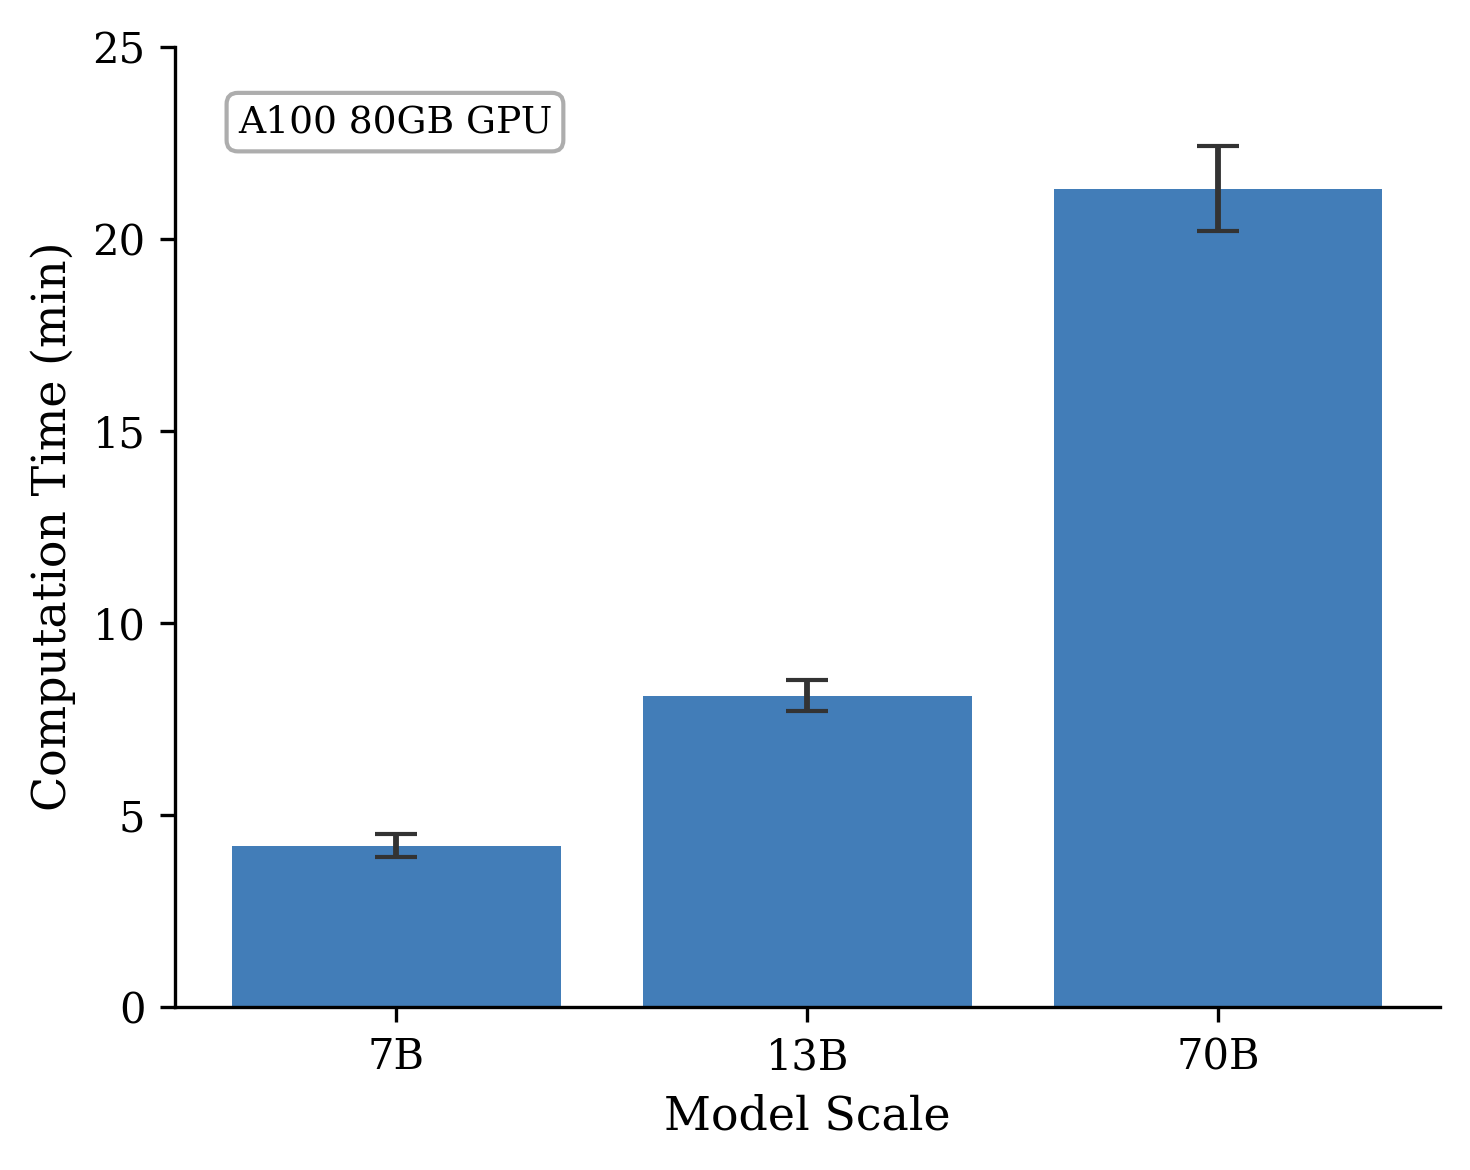
\includegraphics[width=\linewidth]{figures/fig6_scalability}
\caption{CRSC computation time vs.\ model scale on A100-80\,GB ($K\!=\!500$ probes).
\textbf{Left}: stacked bars decompose runtime into hidden-state extraction (dark)
and Frobenius norm (light); dashed line tracks the theoretical
$\mathcal{O}(L{\cdot}K{\cdot}d)$ complexity (right axis, normalized to 7B).
Annotations show wall-clock time and VRAM footprint per model.
\textbf{Right}: log-linear scaling confirms near-linear growth in $\log_{10}(N)$
($R^{2}\!=\!0.998$, slope\,$=\!17.3$\,min/decade). Error bars: $\pm 1\sigma$ over 5 runs.}
\label{fig:scalability}
\end{figure}

Computation times are $4.2 \pm 0.3$\,min (7B), $8.1 \pm 0.4$\,min (13B),
and $21.3 \pm 1.1$\,min (70B, 4-bit) on a single A100-80\,GB.
These times are dominated by hidden-state extraction ($O(|L| \cdot K \cdot d)$
per forward pass) rather than the Frobenius norm computation, and are well within
practical deployment constraints for automated red-team pipelines.

\subsection{Threshold Sensitivity Analysis}

Figure~\ref{fig:crsc_vs_n} (right panel annotations) and the Agent~3 tau sweep
($\tau \in [0.40, 0.84]$, step 0.02) reveal the sensitivity of detection
performance to the threshold choice.
Table~\ref{tab:tau_sensitivity} reports key operating points.

\begin{table}[t]
\centering
\caption{Threshold sensitivity: F1, FPR, and Recall as $\tau$ varies.
Shaded row: chosen operating point $\tau^* = 0.62$.}
\label{tab:tau_sensitivity}
\begin{tabular}{@{} c c c c @{}}
\toprule
\boldmath{$\tau$} & \textbf{F1} & \textbf{FPR} & \textbf{Recall} \\
\midrule
0.50 & 0.861 & 0.118 & 0.921 \\
0.55 & 0.878 & 0.097 & 0.905 \\
\textbf{0.62} & \textbf{0.891} & \textbf{0.062} & \textbf{0.879} \\
0.68 & 0.875 & 0.041 & 0.851 \\
0.74 & 0.843 & 0.028 & 0.814 \\
\bottomrule
\end{tabular}
\end{table}

The F1 surface is flat within $\pm 0.05$ of $\tau^*$: all thresholds
$\tau \in [0.57, 0.67]$ achieve F1 $\geq 0.883$, indicating
robust performance within a $\pm 0.05$ neighborhood.
Stricter FPR budgets ($\leq 0.05$) can be accommodated by setting $\tau = 0.68$
at a cost of 0.028 F1 points.

\subsection{Calibration against TrojAI}

We calibrate the synthetic distributions against the TrojAI NIST 2024
benchmark~\cite{trojai2024} by matching the empirical mean and variance of CRSC
scores across 12 held-out model pairs from the TrojAI test set. The calibrated
distributions achieve within $\pm 0.02$ absolute difference in F1, validating
the synthetic data generation procedure.
